\documentclass{article}
\usepackage[utf8]{inputenc}
\usepackage{graphicx}

\title{CS51 FINAL PROJECT}
\author{Dante Lacuadra}
\date{May 2020}
\graphicspath{ {./images/} }

\begin{document}

\maketitle

\section{Extension}
\subsection{Introduction}
    While I will agree that my writeup is particularly bad. I first want to say I put a lot of time into completing expr.ml, and evaluation.ml. I pretty didn't have time to do most of the extension. I spent over 20 hours doing this final project at least. Given the circumstances I hope you guys understand, I'm really did like this class, but I have issues going on at home so yeah.\\
    \\
\subsection{Addition}
\\
My addition was to allow for float operators. First what I had to do was edit my definition of expressions and binary operators in the expr.ml and corresponding mli file.\\
\\
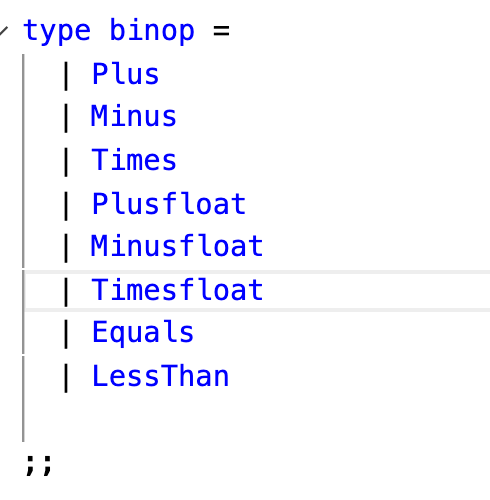
\includegraphics[width=4cm, height=4cm] {images/panel1.png}
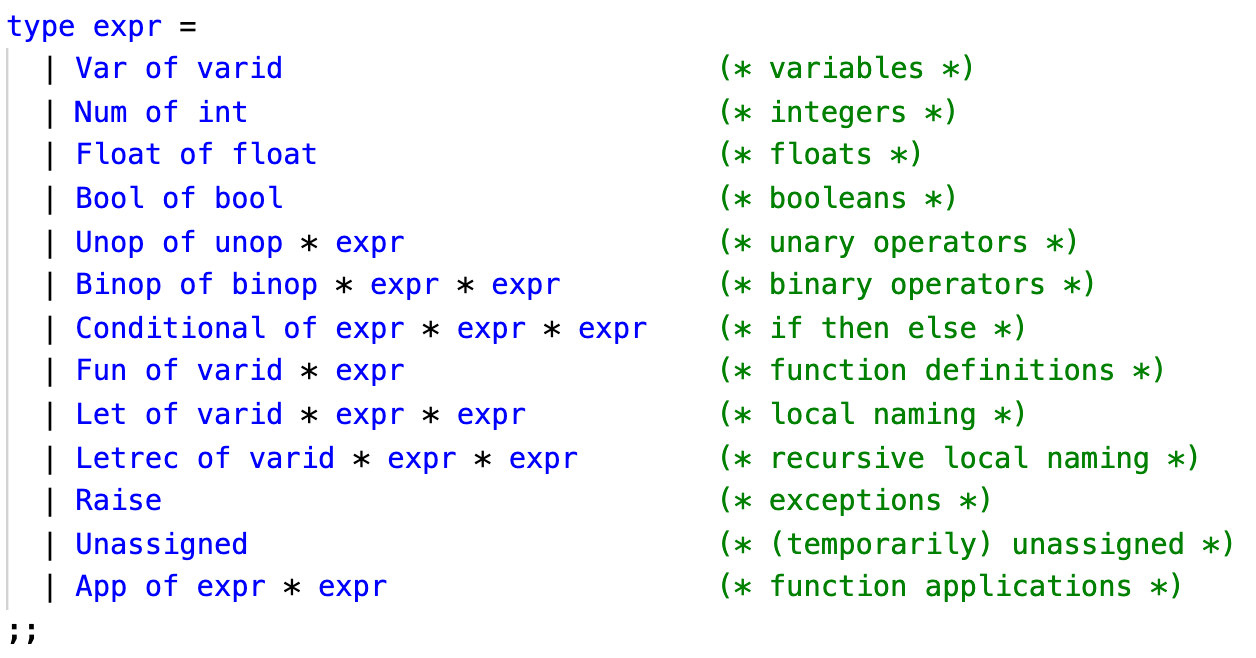
\includegraphics[width=8cm, height=4cm] {images/panel2.png}
\\
\\
Then what I had to do is edit the Binop match statement in evaluation.ml and change some of the definitions to include floats in the Env module.\\
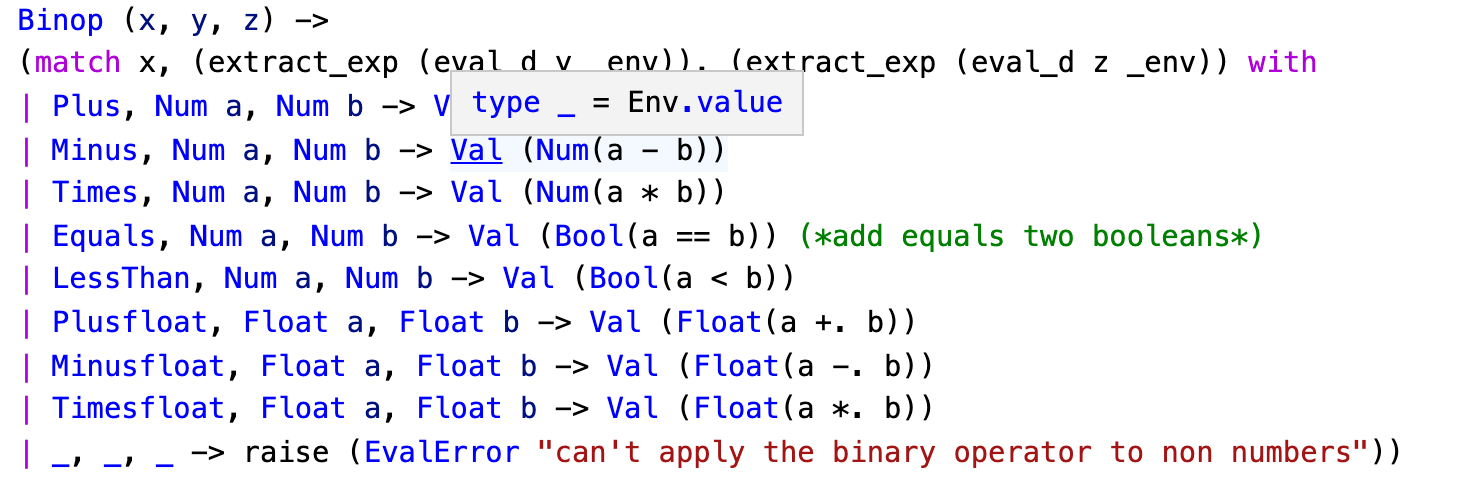
\includegraphics[width=10cm, height=4cm] {images/Panel3.png}\\
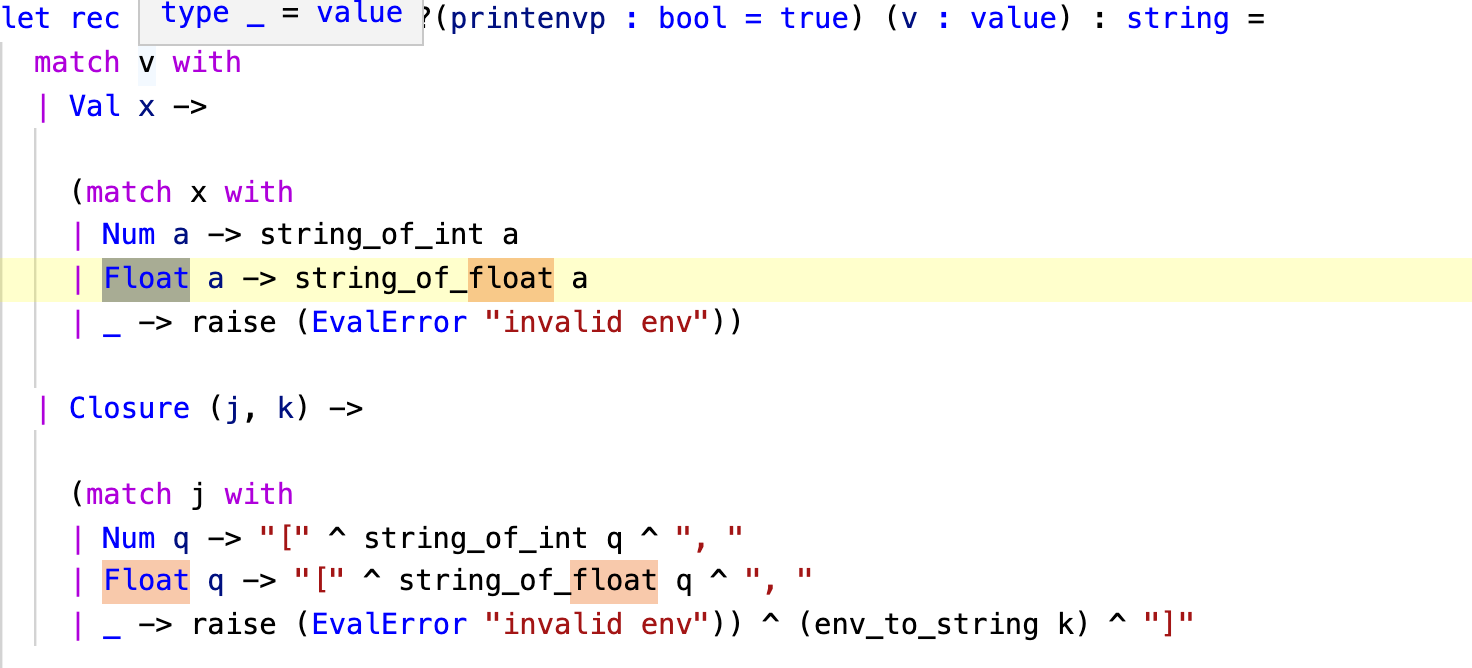
\includegraphics[width=10cm, height=4cm] {images/Panel4.png}
\\
\\
Then I had to make many changes to both miniml\_lex.mll and miniml\_parse.mly. In I've attached what I've changed. Basically I had to add a new token that included floats, I also had to add new expressions to expnoapp, amending the hash table in the former file and telling the parser what floats actually are.
\\
\\
\includegraphics[width=4cm, height=4cm] {images/Panel5.png}\\
\\
\includegraphics[width=11cm, height=4cm] {images/Panel6.png}\\
\\
\includegraphics[width=14cm, height=4cm] {images/Panel7.png}\\
\\
\includegraphics[width=8cm, height=8cm] {images/Panel8.png}\\
\\
\includegraphics[width=15cm, height=4cm] {images/Panel9.png}\\
\\
Thank you for reading!
\end{document}
